\item \textbf{
    Find} \begin{equation*}
    \underset{a\leq x\leq b}{max} f(x) \qquad
    \underset{a\leq x\leq b}{min} f(x) \qquad
    \underset{a\leq x\leq b}{max} |f(x)|
\end{equation*}
\textbf{for the following functions and intervals}
\begin{enumerate}
    \item $f(x)= \frac{2-e^x+2x}{3} \qquad [0,1]$\\
          Calculando la primer y segunda derivada se obtiene lo siguiente:
          \begin{equation*}
              f'(x)= \frac{2-e^x}{3} \qquad f''(x)=\frac{-e^x}{3}
          \end{equation*}
          A partir de la primer derivada podemos obtener los valores criíticos, por lo que se optará por resolver $f'(x_c)=0$. Resultando que ese valor es $x_c=ln(2)$, el cual se encuentra contenido en $[0,1]$, para saber si se trata de un máximo o mínimo de la función se calculará $f''(x_c)$, obteniendo que $f''(ln(2))= -2/3$. Por lo tanto $x_c$ representa un máximo de la función. Grafiando la función en el intervalo $[0,1]$ se obtiene la figura \ref{fig:problema2a}.
          \begin{figure}[H]
              \centering
              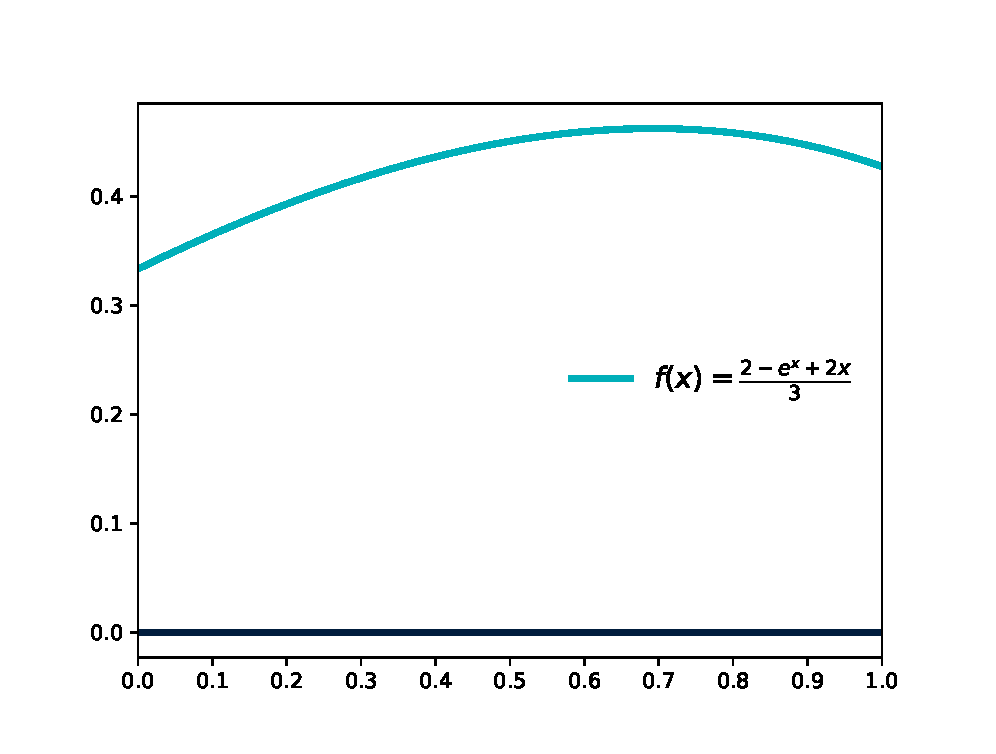
\includegraphics[width=10cm]{Graphics/function_3.eps}
              \caption{función $f(x)= \frac{2-e^x+2x}{3}$ en el intervalo $[0,1]$}
              \label{fig:problema2a}
          \end{figure}
          Verificando así la existencia de $x_c$ dentro del rango. Análiticamente no se puede obtener un mínimo, es por ello que se tomará el valor mínimo o máximo del rango. Siendo este caso el límite inferior. La función es positiva para todo valor en el intervalo, entonces $|f(x)|=f(x)$. Por lo tanto, los valores máximos y mínimos requeridos son:
          \begin{equation*}
              \underset{a\leq x\leq b}{max} f(x)= \frac{2ln(2)}{3} \qquad
              \underset{a\leq x\leq b}{min} f(x) = \frac{1}{3}\qquad
              \underset{a\leq x\leq b}{max} |f(x)| = \frac{2ln(2)}{3}
          \end{equation*}
    \item $f(x)= \frac{4x-3}{x^2-2x} \qquad [0.5,1.5]$\\
          Calculando la primer derivada de la función obtenemos lo siguiente:
          \begin{equation*}
              f'(x)= \frac{-4x^2+6x-6}{(x^2-2x)^2}
          \end{equation*}
          Al obtener los valores críticos se observa que estos son números complejos, entonces no se pueden obtener valores mínimos o máximos análñiticamente. Es por ello que evaluaremos la función en los límites del intervalo. Se realizó la gráfica de la función (figura \ref{fig:problema2b}) para comprobar lo antes dicho. De aqui podemos observar que el valor mínimo y máximo estan en el límite superior e inferior respectivamente.
          \begin{figure}[H]
              \centering
              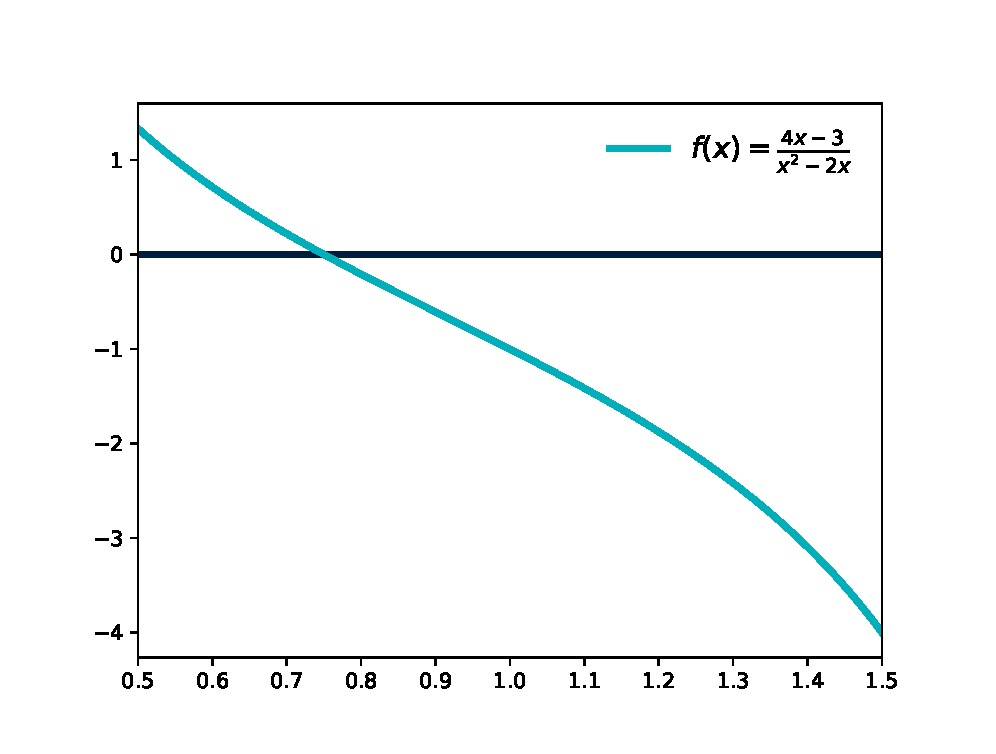
\includegraphics[width=10cm]{Graphics/function_4.eps}
              \caption{Función $f(x)= \frac{4x-3}{x^2-2x}$ en el intervalo $[0.5,1.5]$}
              \label{fig:problema2b}
          \end{figure}
          Por lo tanto
          \begin{equation*}
              \underset{a\leq x\leq b}{max} f(x)= f(0.5)=\frac{4}{3} \qquad
              \underset{a\leq x\leq b}{min} f(x) = f(1.5)=-4
          \end{equation*}
          como $|f(1.5)|>|f(0.5)|$, entonces:
          \begin{align*}
              \underset{a\leq x\leq b}{max} |f(x)| & =|f(1.5)| \\
                                                   & =|-4|     \\
                                                   & =4
          \end{align*}
\end{enumerate}